\subsection{\texorpdfstring{$\ell\Tau$ Channel}{lepton-tau Channel}}
\label{sect:leptonTauCuts}
In lepton ($e$ and $\mu$) $+$ \Tau channels, tight isolated $\Tau$ candidates with $\PT > 20 \GeV$  are selected. To reduce the rate of the fake $\Tau$'s originated from $e$ and $\mu$, the same cut as in the Higgs analysis \cite{CMS_AN_2013-188} is applied on discriminators against $e$ and $\mu$. In $e\Tau$ channel, $\Tau$ objects which pass \emph{MediumElectronMVA3Rejection} against $e$ and the \emph{LooseMuon2Rejection} discriminator against $\mu$ are selected. In the $\mu\Tau$ channel, the tight working point of the \emph{Muon2Rejection} is requested and the Loose working point of the discriminator against electron is applied.

Muons with $\PT > 20 \GeVc$ and $|\eta|<2.1$ are selected in the $\mu\Tau$ channel. The $\mu$'s should pass tight particle flow identification and a tight cut ($<0.1$) on the isolation.
 
In $e\Tau$ channel, each event is requested to have an electron with $\PT >25 \GeVc$ in the $|\eta| < 2.1 $ region. A tight cut of $0.1$ on the isolation and $0.1$ on the $dZ$ of the selected electron are also applied.

To suppress dilepton and multilepton backgrounds, events with an extra $e$ or $\mu$ with $\PT >10 \GeV$ are rejected. In $e\Tau$ channel, for the extra electron to veto, a wider window of $|\eta|<2.3$ is scanned and a looser isolation cut of $0.2$ is applied. To find the extra $\mu$ in this channel, a selection similar to the $\mu$ selection in $\mu\hadtau$ channel is applied. In $\mu\Tau$ channel, events with any extra lepton in $|\eta|<2.4$ region with isolation value $<0.3$ are vetoed. For the extra $\mu$ in this channel, no identification is requested.


After requesting two opposite sign leptons in the events, a loose cut on \MET $(30 \GeV)$ is applied to suppress QCD events. As there is no bquark in the signal, rejecting events with one or more b-tagged jets with $\PT > 20 \GeV$ helps a lot in reducing \ttbar and W+b backgrounds.

To reject QCD low mass resonances, the invariant mass of the lepton and the $\Tau$ is requested to be greater than $15\ \GeV$. Another cut on the invariant mass of the di-lepton system is applied to remove the peak of the \Z+jets events. It has been found that the visible mass of the $Z\to\tau\tau\to\,\ell +\Tau$ moves to $60 \pm 15 GeV$ due to mis-reconstruction of the energy of the $\Tau$ and also the missing energy due to the decay of the $\tau$ to electron. So the events with invariant mass in the range of $[45,75]$ are cut away. The minimum angle in the transverse plane between the \MET and the jets with \PT $>$ 40 \GeVc and $|\eta| <$ 5.0 is asked to be greater than 1.0. As the last pre-selection cut, events with $\mttwo<40 GeV$ are discarded to kill the bulk of the QCD events and get rid of related uncertainties due to mis-modeling and low statistics 
of the QCD events. As it has mentioned above, the signal events are expected to have high \mttwo values and are not removed with such a cut.

\begin{table}
\begin{center}
\begin{tiny}
\begin{tabular}{llllllllll}
\hline
\hline
  & SUSY(380,1) & QCD & W & ZX & Top & WW & Higgs & MC & Data \\
\hline
\hline
\MET,b,DiLepton Selection & 20.49$\pm$2.03 & 6748.66 & 46139.56 & 17071.56 & 1845.78 & 589.41 & 248.92 & 72643.89$\pm$2147.82 & 76066.00$\pm$275.80 \\
Extra Lepton Veto & 19.89$\pm$2.00 & 6476.83 & 46048.34 & 15902.83 & 1797.65 & 575.12 & 243.94 & 71044.71$\pm$2130.46 & 74382.00$\pm$272.73 \\
Z veto & 15.99$\pm$1.71 & 4788.17 & 27465.97 & 5826.98 & 1355.28 & 437.13 & 155.56 & 40029.09$\pm$2068.14 & 41968.00$\pm$204.86 \\
$\mindphifour > 1.0$ & 12.70$\pm$1.56 & 2271.96 & 11416.01 & 3169.72 & 693.16 & 198.61 & 94.85 & 17844.31$\pm$1498.73 & 19761.00$\pm$140.57 \\
$\mttwo > 40 \GeV$ & 9.86$\pm$1.38 & 1514.64 & 4466.3 & 68.9 & 251.07 & 82.14 & 1.46 & 6384.52$\pm$1478.31 & 5446.00$\pm$73.80 \\
\hline
$\mttwo > 90 \GeV$ & 5.69$\pm$1.08 & 0 & 16.18 & 1.82 & 0.64 & 1.57 & 0.19 & 20.40$\pm$4.24 & - \\
$\tauMT > 200 \GeV$ & 3.47$\pm$0.88 & 0 & 1.29 & 0.38 & 0.02 & 0.05 & 0.06 & 1.79$\pm$0.63 & - \\

\hline
\hline
\end{tabular}
\caption{Cut-flow-table for $e\hadtau$ channel. Only statistical uncertainties are reported.}
\label{tbl:cutflowtableeletau}
\end{tiny}
\end{center}
\end{table}

\begin{table}
\begin{center}
\begin{tiny}
\begin{tabular}{llllllllll}
\hline
\hline
  & SUSY(380,1) & QCD & W & ZX & Top & WW & Higgs & MC & Data \\
\hline
\hline
\MET,b,DiLepton Selection & 16.71 & 6791.27 & 79084.31 & 37000.63 & 4433.53 & 1778.41 & 242.76 & 129330.9$\pm$3009.89 & 121644 \\
Extra Lepton Veto   & 14.92 & 5192.66 & 77139.4 & 32166.18 & 2972.25 & 1034.93 & 217.98 & 118723.39$\pm$2601.51 & 111344 \\
Z Veto              & 12.69 & 1721.45 & 46551.75 & 6963.01 & 2128.4 & 759.7 & 109.29 & 58233.6$\pm$1262.89 & 55282 \\
$\mindphifour > 1.0$ & 10.22 & 70.87 & 19592.59 & 4130.47 & 1129.26 & 382.9 & 80.08 & 25386.17$\pm$214.76 & 26955 \\ 
$\mttwo > 40 \GeV$  & 7.38 & 0 & 8558.78 & 157.33 & 427.51 & 164.59 & 1.5 & 9309.72$\pm$132.94 & 9253 \\\hline
$\mttwo > 90 \GeV$ & 3.48 & 0 & 17.67 & 1.17 & 1.15 & 2.19 & 0.17 & 22.35$\pm$5.2 & - \\
$\tauMT > 200 \GeV$ & 2.09 & 0 & 0.79 & 0.28 & 0 & 0.34 & 0.05 & 1.45$\pm$.49 & - \\
\hline
\hline
\end{tabular}
\caption{Cut-flow-table for $\mu\hadtau$ channel. The uncertainties are just statistical.}
\label{tbl:cutflowtablemuotau}
\end{tiny}
\end{center}
\end{table}

The cut-flow-tables for the $e\Tau$ and $\mu\Tau$ pre-selections are shown in tables~\ref{tbl:cutflowtableeletau} and~\ref{tbl:cutflowtablemuotau} respectively. The distribution of the \PT of the $\Tau$ and \MET in the pre-selected events in both channels are shown in figures~\ref{fig:datamceletau} and~\ref{fig:datamcmuotau} . The good agreement between data and MC confirms that the needed correction factors are considered carefully.

\begin{figure}[htbp]
\centering
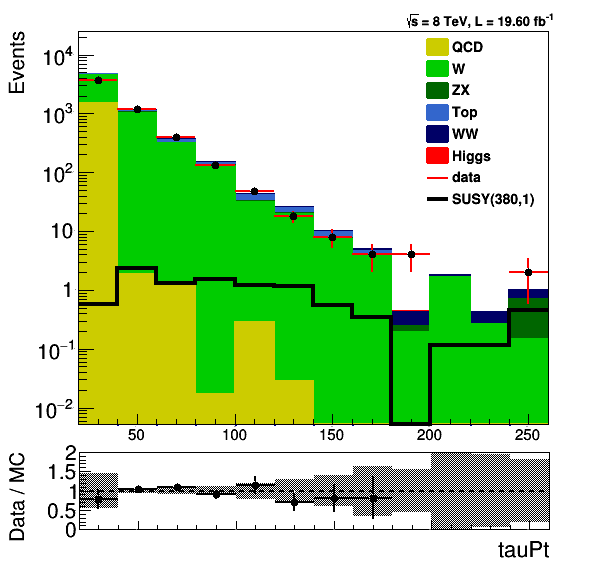
\includegraphics[angle=0,scale=0.35]{SelectionEleTau/TauPt.png}
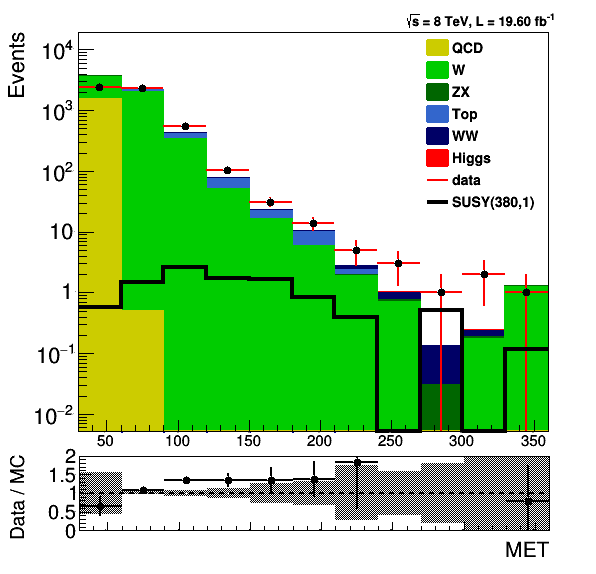
\includegraphics[angle=0,scale=0.35]{SelectionEleTau/MET.png}
\caption{Left: \Tau\PT. Right: \MET in reselected $e\hadtau$ events.}
\label{fig:datamceletau}
\end{figure}

\begin{figure}[htbp]
\centering
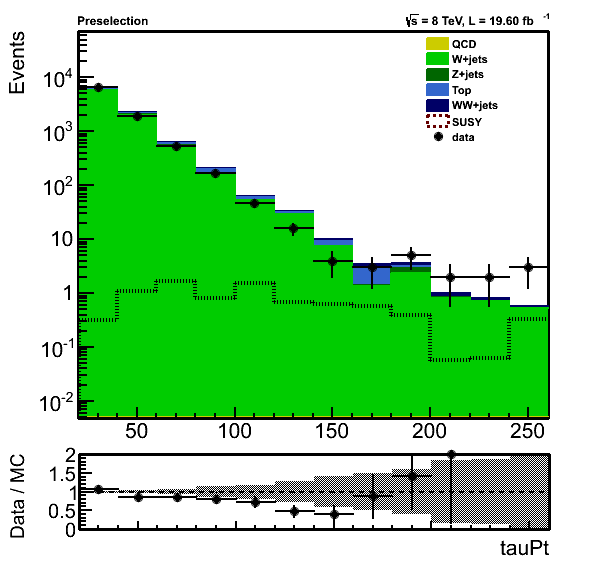
\includegraphics[angle=0,scale=0.35]{SelectionMuTau/tauPt_muTau.png}
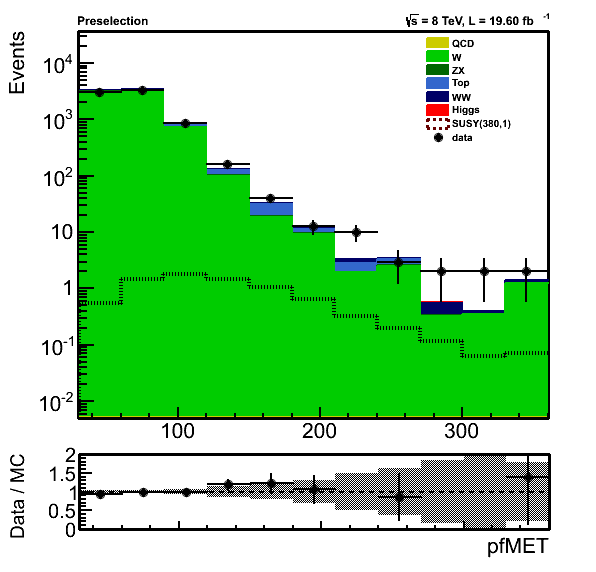
\includegraphics[angle=0,scale=0.35]{SelectionMuTau/pfMET_muTau.png}
\caption{Left: \Tau\PT. Right: \MET in preselected $\mu\hadtau$ events.}
\label{fig:datamcmuotau}
\end{figure}

Similar to the $\Tau\Tau$ channel, first we find the optimized cut on the \mttwo to suppress backgrounds especially W+jet events. As it has been shown in figure~\ref{fig:mt2leptontau}, the best value to cut on, similar to the $\Tau\Tau$ channel is $\mttwo > 90 \GeV$ for both $\ell\Tau$ channels. Such a high cut on the \mttwo increases the sensitivity of the study to signal events with high $\chipm$ and $\chiz$ mass differences. We then investigate the shape of different variables for signal and backgrounds and try to find the most optimized cut to have the best exclusion. The most sensitive variable for both channels are found to be the $\Tau$ transverse mass. As it has been shown in figure~\ref{fig:taumtleptontau}, the best cut value for the high mass difference signal is $\tauMT > 200 \GeV$. The composition of the backgrounds and number of remaining signals for both channels can be found in the last row of the cut-flow-tables (tables~\ref{tbl:cutflowtableeletau} and~\ref{tbl:cutflowtablemuotau}).

\begin{figure}[htbp]
\centering
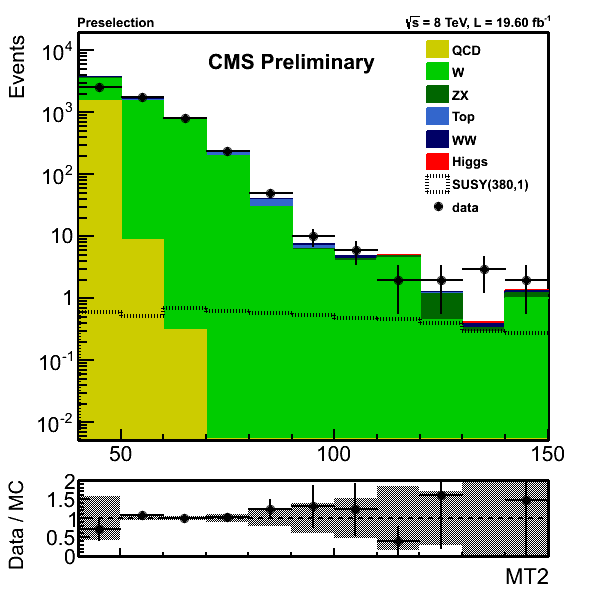
\includegraphics[angle=0,scale=0.35]{SelectionEleTau/MT2.png}
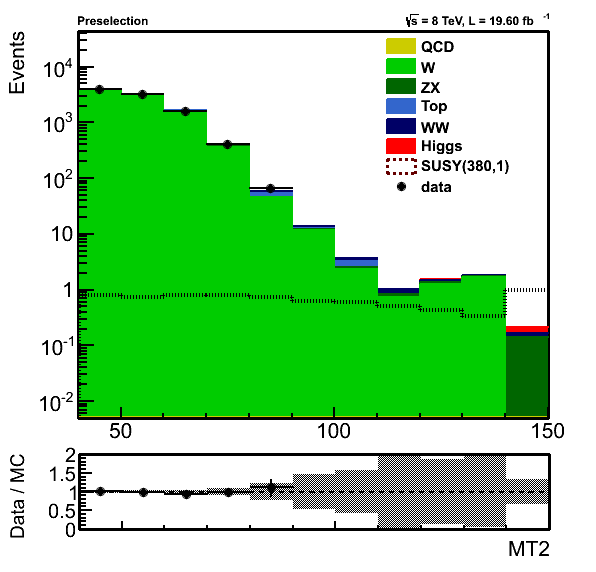
\includegraphics[angle=0,scale=0.35]{SelectionMuTau/MT2_muTau.png}
\caption{\mttwo distribution of preselected events in (Left) $e\hadtau$ and (Right) $\mu\hadtau$ channels.}
\label{fig:mt2leptontau}
\end{figure}

\begin{figure}[htbp]
\centering
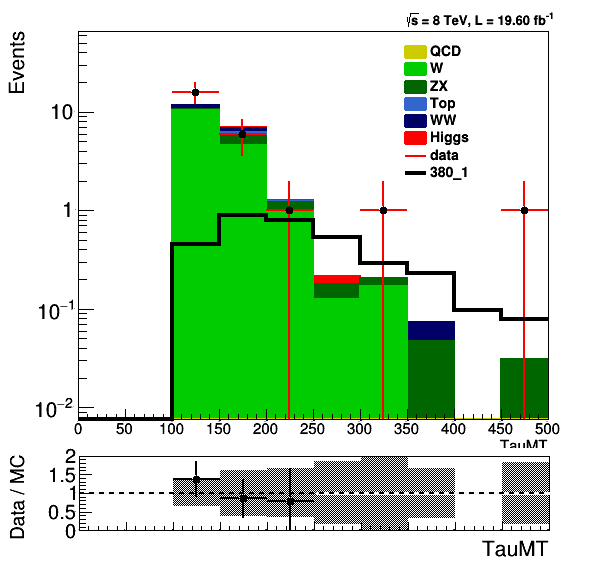
\includegraphics[angle=0,scale=0.35]{SelectionEleTau/TauMT.png}
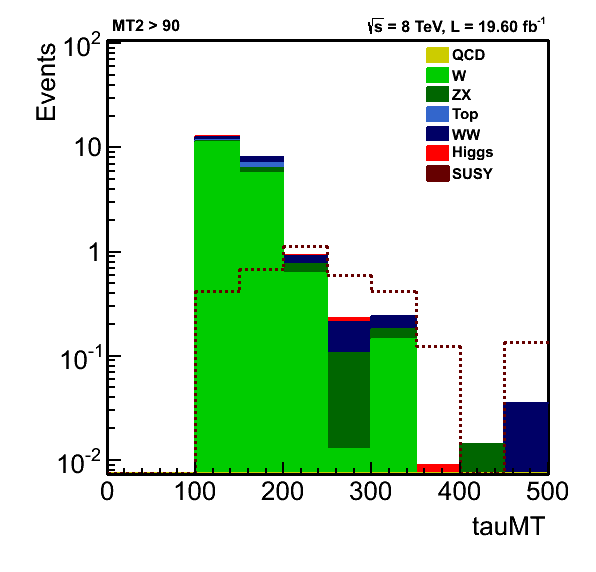
\includegraphics[angle=0,scale=0.35]{SelectionMuTau/tauMT_MuTau.png}
\caption{\tauMT distribution for events with $\mttwo>90\GeV$ in (Left) $e\hadtau$ and (Right) $\mu\hadtau$ channels.}
\label{fig:taumtleptontau}
\end{figure}
Opposite to the $\Tau\Tau$ channel, the events with $\mttwo<90 \GeV$ are not useful in $\ell\Tau$ channels because of the contamination of 
the W+jets events. It was investigated if increasing the \pt of the objects can increase the sensitivity in this bin, but no improvment was seen.
